\documentclass[tikz,border=8pt]{standalone}
% Shared TikZ style for synorg platform diagrams. Each diagram \input's this
% inside a standalone document. Palette tracks the Material "teal" site theme so
% figures read as one system in light mode (SVGs are theme-neutral otherwise).
\usetikzlibrary{arrows.meta,positioning,shapes.geometric,fit,backgrounds,calc,decorations.pathreplacing}

\definecolor{synteal}{HTML}{00897B}   % primary
\definecolor{synfill}{HTML}{E0F2F1}   % light fill
\definecolor{synamber}{HTML}{B26A00}  % warning / lend
\definecolor{synred}{HTML}{B00020}    % deny / danger
\definecolor{syngrey}{HTML}{5F6368}   % muted

\tikzset{
  >=Stealth,
  font=\sffamily\small,
  box/.style={draw=synteal,line width=0.6pt,rounded corners=2pt,fill=synfill,
              inner sep=5pt,align=center},
  plane/.style={draw=synteal,line width=0.8pt,rounded corners=3pt,fill=synfill,
                inner sep=8pt,align=center},
  state/.style={draw=synteal,line width=0.7pt,circle,fill=synfill,inner sep=3pt,
                minimum size=11mm,align=center,font=\sffamily\footnotesize},
  decision/.style={draw=synteal,line width=0.7pt,diamond,aspect=2,fill=synfill,
                   inner sep=1pt,align=center,font=\sffamily\footnotesize},
  deny/.style={draw=synred,fill=synred!8,text=synred},
  warn/.style={draw=synamber,fill=synamber!10},
  flow/.style={->,line width=0.6pt,draw=syngrey},
  flowlbl/.style={font=\sffamily\footnotesize,text=syngrey,inner sep=2pt},
  note/.style={font=\sffamily\footnotesize\itshape,text=syngrey},
}

\begin{document}
% Cluster anatomy (architecture.md "Anatomy of the estate"): the two EKS
% clusters as deployed today — synorg-mgmt (hub, ArgoCD only) and synorg-pilot
% (spoke, all workloads), with the namespaces each one actually runs and the
% region-level capacity objects (held ODCRs, checkpoint bucket) the pilot
% draws on. Names come from infra/terraform/* and clusters/*.
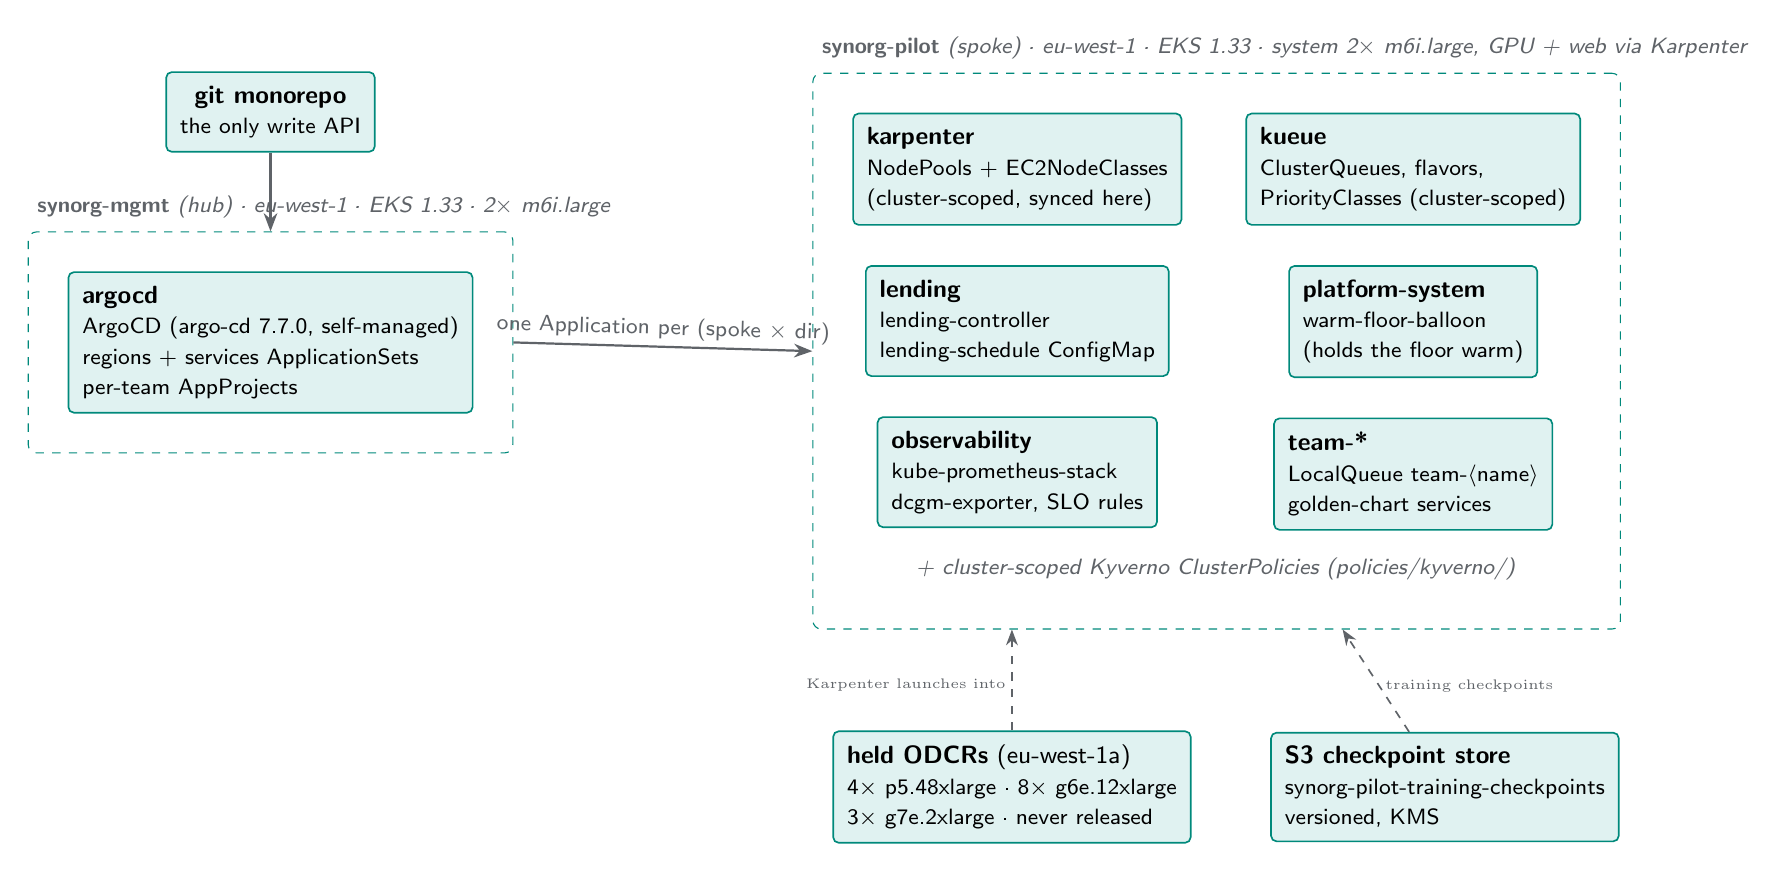
\begin{tikzpicture}[node distance=6mm and 10mm]

  % ---- hub cluster ----
  \node[box,align=left] (argons)
    {\textbf{argocd}\\\footnotesize ArgoCD (argo-cd 7.7.0, self-managed)\\\footnotesize regions + services ApplicationSets\\\footnotesize per-team AppProjects};
  \begin{scope}[on background layer]
    \node[draw=synteal,dashed,rounded corners=3pt,inner sep=5mm,
          fit=(argons)] (mgmt) {};
  \end{scope}
  \node[note,anchor=south west] at ($(mgmt.north west)+(0mm,0.5mm)$)
    {\textbf{synorg-mgmt} (hub) · eu-west-1 · EKS 1.33 · 2$\times$ m6i.large};

  % ---- git, feeding the hub ----
  \node[box,above=10mm of mgmt] (git)
    {\textbf{git monorepo}\\\footnotesize the only write API};
  \draw[flow,line width=0.8pt] (git) -- (mgmt);

  % ---- spoke cluster: namespace grid ----
  \node[box,align=left] (kar) at ($(mgmt.east)+(64mm,22mm)$)
    {\textbf{karpenter}\\\footnotesize NodePools + EC2NodeClasses\\\footnotesize (cluster-scoped, synced here)};
  \node[box,align=left,right=8mm of kar] (kue)
    {\textbf{kueue}\\\footnotesize ClusterQueues, flavors,\\\footnotesize PriorityClasses (cluster-scoped)};
  \node[box,align=left,below=5mm of kar] (lend)
    {\textbf{lending}\\\footnotesize lending-controller\\\footnotesize lending-schedule ConfigMap};
  \node[box,align=left,below=5mm of kue] (plat)
    {\textbf{platform-system}\\\footnotesize warm-floor-balloon\\\footnotesize (holds the floor warm)};
  \node[box,align=left,below=5mm of lend] (obs)
    {\textbf{observability}\\\footnotesize kube-prometheus-stack\\\footnotesize dcgm-exporter, SLO rules};
  \node[box,align=left,below=5mm of plat] (team)
    {\textbf{team-*}\\\footnotesize LocalQueue team-$\langle$name$\rangle$\\\footnotesize golden-chart services};
  \node[note] (kyv) at ($(obs.south east)!0.5!(team.south west)+(0mm,-5mm)$)
    {+ cluster-scoped Kyverno ClusterPolicies (policies/kyverno/)};
  \begin{scope}[on background layer]
    \node[draw=synteal,dashed,rounded corners=3pt,inner sep=5mm,
          fit=(kar)(kue)(lend)(plat)(obs)(team)(kyv)] (pilot) {};
  \end{scope}
  \node[note,anchor=south west] at ($(pilot.north west)+(0mm,0.5mm)$)
    {\textbf{synorg-pilot} (spoke) · eu-west-1 · EKS 1.33 · system 2$\times$ m6i.large, GPU + web via Karpenter};

  % ---- region-level capacity the pilot draws on ----
  \node[warn,box,align=left] (odcr) at ($(pilot.south)+(-26mm,-20mm)$)
    {\textbf{held ODCRs} (eu-west-1a)\\\footnotesize 4$\times$ p5.48xlarge · 8$\times$ g6e.12xlarge\\\footnotesize 3$\times$ g7e.2xlarge · never released};
  \node[box,align=left,right=10mm of odcr] (s3)
    {\textbf{S3 checkpoint store}\\\footnotesize synorg-pilot-training-checkpoints\\\footnotesize versioned, KMS};
  \draw[flow,dashed] (odcr) -- node[flowlbl,left,font=\tiny,pos=0.45]{Karpenter launches into} ($(pilot.south)+(-26mm,0mm)$);
  \draw[flow,dashed] (s3) -- node[flowlbl,right,font=\tiny,pos=0.45]{training checkpoints} ($(pilot.south)+(16mm,0mm)$);

  % ---- hub -> spoke sync ----
  \draw[flow,line width=0.8pt] (mgmt.east) -- node[flowlbl,above,sloped]
    {one Application per (spoke $\times$ dir)} (pilot.west);
\end{tikzpicture}
\end{document}
